\documentclass[10pt]{article}
\usepackage{icmlko}

\icmlmeta{IP 파운데이션 월드모델}{171}{일관성과 정확성이 갈린다}{걸음 불변 칸으로 정식화를 가를 수 있는지 물었다. 갈린다 --- 그런데 일관성으로 세운 순위와 정확성으로 세운 순위가 정반대다}

\begin{document}

\twocolumn[
\icmlheader

\begin{abstract}
노트 162가 ``18칸으로는 정식화를 못 가른다''고 하고 노트 170이 걸음 불변
칸 28개를 만들었다. 가를 수 있나. \textbf{잣대를 바꾸면 갈린다.} 다섯
정식화에서 \textbf{걸음 불변 칸의 \emph{비율}} 이 78\%$\sim$100\%로
\textbf{폭 0.222} 다 --- 노트 162가 고른 상위절반(0.056)의 네 배이고,
36칸에서 $p{\approx}0.9$ 의 $2\,\mathrm{se}$(0.10)를 처음으로 넘는다. 판과의
순위상관이 $-$0.791이고 씨앗 순위 일치가 $+$0.973이다. \textbf{그리고 이
잣대는 라벨도 사전 부호도 안 본다} --- ``걸음을 바꿔도 같은 답을 내나''만
묻는다. \textbf{그런데 여기서 멈추면 안 된다.} 같은 불변 칸에서 \emph{정확도}
를 재면 순위가 뒤집힌다 --- F18 배깅 · F8 부스팅이 \textbf{93\%}이고 선형
셋이 75$\sim$89\%다(판과 $+$0.564). \textbf{이건 잣대가 아니라 조건화의
산물이다} --- 트리는 불변 칸이 78\%뿐이고 그 골라낸 28칸이 깨끗한 것이고,
선형은 100\%가 불변이라 애매한 칸까지 다 들어간다. 분모가 다른 두 수를
견준 것이다. 분해하면 맞는다: 전체 정확도 $=$ 불변비율 $\times$ 불변정확
$+$ 흔들비율 $\times$ 흔들정확이고, F18은 $0.78{\times}0.93 +
0.22{\times}0.50 = 83\%$, F9 순위우도는 $1.00{\times}0.89 = 89\%$다.
\textbf{읽는 법은 이렇다 --- 선형은 고루 맞히고 트리는 몰아 맞힌다.}
트리는 자기가 어느 답을 믿어도 되는지 알려 주는 대신(불변 28칸 93\%) 나머지
8칸에서 동전이고, 선형은 전 칸에서 89\%로 고르다. \textbf{둘 중 무엇이
나은지는 쓰임이 정한다} --- 한 기획서에 답을 줘야 하면 트리의 ``이 칸은
못 믿는다''가 값지고, 전 도메인 평균이 필요하면 선형이 낫다.
\end{abstract}
]

\begin{figure*}[t]
\centering
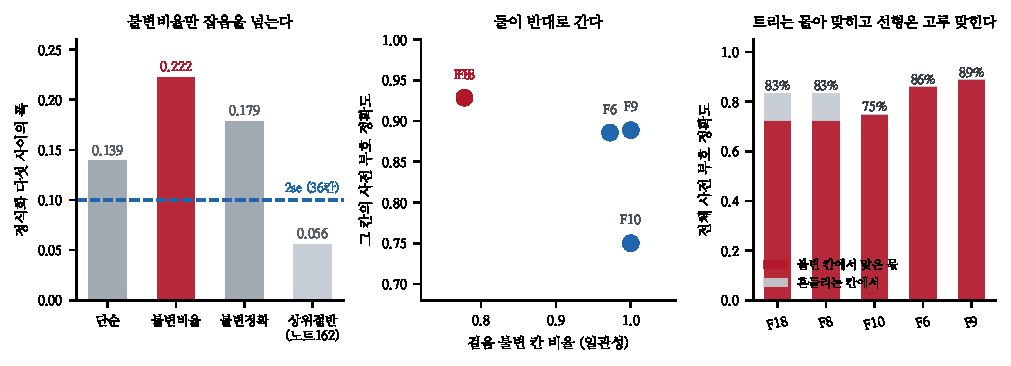
\includegraphics[width=\textwidth]{figs/consist.pdf}
\caption{왼쪽 --- 불변비율만 잡음을 넘는다. 가운데 --- 일관성과 정확성이
반대로 간다. 오른쪽 --- 트리는 몰아 맞히고 선형은 고루 맞힌다.}
\end{figure*}

\section{불변비율은 가른다}

\begin{table}[t]
\centering\tsize
\caption{손잡이 잣대 넷. 폭 · 판과의 상관 · 씨앗 안정.}
\begin{tabular}{lrrr}
\toprule
& 폭 & 판상관 & 씨앗 \\
\midrule
단순 & .139 & $-$.667 & $+$1.000 \\
\textbf{불변비율} & \textbf{.222} & $-$.791 & $+$.973 \\
불변정확 & .179 & $+$.564 & $+$.975 \\
상위절반 (노트 162) & .056 & $-$.866 & $+$1.000 \\
\midrule
\textbf{$2\,\mathrm{se}$ (36칸)} & \textbf{.100} & & \\
\bottomrule
\end{tabular}
\end{table}

\claimx{\textbf{불변비율이 처음으로 잡음을 넘는다.} 폭 0.222가 36칸
$2\,\mathrm{se}$ 0.100의 두 배다. 노트 162가 고른 상위절반은 0.056으로
1 se 였다.}{게다가 이 잣대는 라벨도 사전 부호도 안 본다 --- ``걸음을 0.05
에서 1.0까지 바꿔도 같은 부호를 내나''만 묻는다. \textbf{순환이 원천적으로
없다.}}

\begin{table}[t]
\centering\tsize
\caption{정식화 다섯.}
\begin{tabular}{lrrrr}
\toprule
& 판 $\rho$ & 불변비율 & 불변정확 & 전체 \\
\midrule
F18 배깅 & \textbf{$+$.4491} & 78\% & \textbf{93\%} & 83\% \\
F8 부스팅 & $+$.4341 & 78\% & \textbf{93\%} & 83\% \\
F10 도메인수축 & $+$.3735 & \textbf{100\%} & 75\% & 75\% \\
F6 능형 & $+$.3671 & 97\% & 89\% & 86\% \\
F9 순위우도 & $+$.3519 & \textbf{100\%} & 89\% & \textbf{89\%} \\
\bottomrule
\end{tabular}
\end{table}

\section{그런데 정확도로 세우면 뒤집힌다}

\claimx{\textbf{불변정확의 판상관이 $+$0.564다} --- 다른 셋과 반대 방향이다.
트리 둘이 93\%로 제일 높다.}{여기서 ``역시 부스팅이 손잡이도 낫다''로
읽으면 안 된다.}

\claimx{\textbf{조건화의 산물이다.} 트리는 불변 칸이 78\%뿐이라 \emph{골라낸}
28칸을 채점하고, 선형은 100\%가 불변이라 애매한 칸까지 36칸을 다 채점한다.
\textbf{분모가 다른 두 수를 견준 것이다.}}{노트 162가 상위절반을 고를 때
같은 함정을 피했었다 --- 그때는 모든 정식화가 같은 18칸을 썼다. 이번엔
필터가 정식화마다 다르다.}

\begin{table}[t]
\centering\tsize
\caption{분해. 전체 $=$ 불변$\times$정확 $+$ 흔들$\times$정확.}
\begin{tabular}{lrrr}
\toprule
& 불변에서 & 흔들에서 & 전체 \\
\midrule
F18 배깅 & $.78{\times}.93$ & $.22{\times}.50$ & 83\% \\
F6 능형 & $.97{\times}.89$ & $.03{\times}.00$ & 86\% \\
F9 순위우도 & $1.0{\times}.89$ & --- & \textbf{89\%} \\
F10 도메인수축 & $1.0{\times}.75$ & --- & 75\% \\
\bottomrule
\end{tabular}
\end{table}

\section{선형은 고루, 트리는 몰아}

\claimx{\textbf{트리는 자기가 어느 답을 믿어도 되는지 알려 준다} --- 불변
28칸에서 93\%, 나머지 8칸에서 50\%(동전)다. \textbf{선형은 전 칸에서
89\%로 고르다.}}{F10 도메인수축은 100\% 불변인데 75\%다 --- \textbf{일관되게
틀릴 수도 있다.} 일관성은 정확성의 보증이 아니다.}

\claimx{\textbf{둘 중 무엇이 나은지는 쓰임이 정한다.} 한 기획서에 답을
줘야 하면 ``이 칸은 못 믿는다''는 정보가 값지고(트리), 전 도메인 평균이
필요하면 고른 쪽이 낫다(선형).}{이 판의 순위표는 판 $\rho$ 하나로 세우니
그 구분을 못 담는다. 노트 144 · 146 · 147 · 159 · 170에 이어 여섯 번째로
같은 결론이다 --- \textbf{한 숫자로는 못 담는다.}}

\begin{table}[t]
\centering\tsize
\caption{남은 것.}
\begin{tabular}{ll}
\toprule
공통 칸 & 다섯 정식화가 다 불변인 칸으로 다시 재면 \\
F10 & 100\% 일관되게 75\% --- 무엇을 일관되게 틀리나 \\
\textbf{쓰임} & 기획서 한 건에 답할 때의 정확도를 따로 잰다 \\
\bottomrule
\end{tabular}
\end{table}

첫 줄이 공정한 비교다. 다섯 정식화가 \emph{모두} 불변인 칸만 골라 채점하면
분모가 같아지고 조건화가 사라진다. 그 칸이 몇이고 거기서 순위가 어떻게
되는지가 다음이다.

\end{document}
